%\jg{The goal of this section is two fold, one introduce basic
%  concepts needed further ahead}

In this class we will introduce several fundamental concepts needed further ahead. We start with an introduction to Python, the programming language we will use in the lab sessions. Afterwards, we present several notions on probability theory and linear algebra. Finally, we focus on numerical optimization. 

The goal of this class is to give you the basic knowledge for you to understand the following lectures. We will not enter in too much detail in any of the topics. 


\section{Python}
\subsection{Python Basics}

\subsubsection{Running Python code}

We will start by creating and running a dummy program in Python which simply prints the ``Hello World!'' message to the standard output (this is usually the first program you code when learning a new programming language). 

There are two main ways in which you can run code in Python: 

\begin{description}
\item[From a file]--~~Create a file named \texttt{yourfile.py} and write your program in it, using your favorite text editor:

\begin{python}
print 'Hello World!'
\end{python}

After saving and closing the file, you can run your code by calling: 

\begin{verbatim}
python yourfile.py
\end{verbatim}

in the command line. This will run the program and display the message ``Hello World!''. After, the control will return to the command line.




\item[In the interactive command line]--~~Start the interactive command line in Python using the command \texttt{python}. After this, you can run Python code by simply writing it and pressing enter. In our lab sessions, we will use Python in interactive mode several times. The standard Python interface is not very friendly, though. IPython, which stands for \emph{interactive Python}, is an improved Python shell. It saves your command history between sessions, has basic auto-complete, and has internal support for interacting with graphs through matplotlib. IPython is also designed to facilitate running parallel code on clusters of machines, but we will not make use of that functionality.

To run IPython, simply type \texttt{ipython} on your command line\footnotemark\footnotetext{Note that in some systems, e.g. Linux, you may need to run the command lower-cased.}. For interactive numeric use, the \texttt{--pylab} flag imports numpy and matplotlib (the two libraries we will extensively use in the lab sessions) for you and sets up interactive graphs:

\begin{verbatim}
IPython --pylab
\end{verbatim}

You can then run Python commands in the IPython command line

\begin{python}
 In[]: print "Hello, World!"
Out[]: Hello, World!
\end{python}

but you can also run Python code written into a file.

\begin{python}
 In[]: run ./yourfile.py
Out[]: Hello, World!
\end{python}
\end{description}


%The first program in every new language is usually a program printing the "Hello World" message.



Keep in mind that you can easily switch between these two modes. You can quickly test commands in the command line directly and e.g. inspect variables. Larger sections of code can be stored and run from files.

\subsubsection{Help and Documentation}

There are several ways to get help on IPython:

\begin{itemize}
\item Adding a question mark to the end of a function or variable and pressing Enter brings up associated documentation. Unfortunately, not all packages are well documented. Numpy and matplotlib are pleasant exceptions;
% It probably does not work because print is a special keyword, unlike Python 3. 
% Since we are using 2.7 we should have help("__builtin__.print") instead.
% However, since help("if") gives the correct information, I'm changing this.
\item \code{help('if')} gets the online documentation for the \code{if} keyword;
\item \code{help()}, enters the help system.
\item When at the help system, type \code{q} to exit.
\end{itemize}

\noindent For more information on IPython~\citep{PER-GRA:2007}, check the website: \url{http://ipython.scipy.org/moin/}

\subsubsection{Exiting}

Exit IPython by typing \code{exit()} or \code{quit()} (or typing CTRL-D).

\subsection{Python by Example}

\subsubsection{Basic Math Operations}

Python supports all basic arithmetic operations, including exponenation. For example, the following code:
\begin{python}
print 3 + 5
print 3 - 5
print 3 * 5
print 3 / 5
print 3 ** 5
\end{python}

\noindent will produce the following output:
\begin{python}
8
-2
15
0
243
\end{python}

Notice that division is always considered as integer division, hence the result being 0 on the example above. To force a floating point division you can force one of the operands to be a floating point number:
\begin{python}
print 3 / 5.0
0.6
\end{python}

Also, notice that the symbol \texttt{**} is used as exponentation operator, unlike other major languages which use the symbol \texttt{\^}. In fact, the \texttt{\^} symbol has a different meaning in Python (bitwise XOR) so, in the beginning, be sure to double-check your code if it uses exponentiation and it is giving unexpected results.

\subsubsection{Data Structures}

In Python, you can create lists of items with the following syntax:

\begin{python}
countries = ['Portugal','Spain','United Kingdom']
\end{python}

A string should be surrounded with apostrophes (') or quotes (``). You can access a list with
the following:

\begin{itemize}
 \item \code{len(L)}, which returns the number of items in L;
 \item \code{L[i]}, which returns the item at index $i$ (the first item has index 0);
 \item \code{L[i:j]}, which returns a new list, containing all the items between indexes $i$ and $j-1$, inclusive. 
\end{itemize}

\begin{exercise}
 Use L[i:j] to return the countries in the Iberian Peninsula.
\end{exercise}

\subsubsection{Loops and Indentation}

A loop allows a section of code to be repeated a certain number of times, until a stop condition is reached. For instance, when the list you are iterating has reached its end or when a variable has reached a certain value (in this case, you should not forget to update the value of that variable inside the code of the loop). In Python you have \code{while} and \code{for} loop statements. The following two example programs output exactly the same using both statements: the even numbers from 2 to 8.

\begin{python}
i = 2
while i < 10:
  print i  
  i += 2 
\end{python}

\begin{python}
for i in range(2,10,2):
    print i
\end{python}

You can copy and run this from the IPython command line. Alternatively you can write this into your \texttt{yourfile.py} file an run it as well. Notice something? It is possible that the code did not act as expected or maybe an error message popped up. This brings us to an important aspect of Python: \textbf{indentation}. Indentation is the number of blank spaces at the leftmost of each command. This is how Python differentiates between blocks of commands inside and outside a statement, e.g. \code{while}, \code{for} or other. All commands within a statement have the same number of blank spaces at their leftmost. For instance, consider the following code: 

\begin{python}
a=1
while a <= 3:
    print a
    a += 1
\end{python}

\noindent and its output:

\begin{python}
1
2
3
\end{python}


\begin{exercise}
Can you then predict the output of the following code?:

\begin{python}
a=1
while a <= 3:
    print a
a += 1
\end{python}

\end{exercise}

\noindent Bear in mind that indentation is often the main source of errors when starting to work with Python. Try to get used to it as quickly as possible. It is also recommendable that you use a text editor that can display all characters e.g. blank space, tabs, since these characters can be visually similar but are considered different by Python. One of the most common mistakes by newcomers to Python is to have their files indented with spaces on some lines and with tabs on other lines. Visually it might appear that all lines have proper indentation, but you will get an \texttt{IndentationError} message if you try it. The recommended\footnote{The PEP8 document (\texttt{www.python.org/dev/peps/pep-0008}) is the official coding style guide for the Python language.} way is to use 4 spaces for each indentation level.

%The \code{range} function is built into Python and it creates lists containing arithmetic progressions. 

%\begin{exercise}
%David, John, Allysson and Anne are four of your colleagues in the Summer Course. Create a python program to greet all of them. The output should be\\
%\begin{python} 
%Hello, David!
%Hello, John!
%Hello, Allysson!
%Hello, Anne!
%\end{python}
%Note that you have around 100 colleagues. You should use the data structures you have just learned to minimize the lines of code you are using in this exercise.
%\end{exercise}

\subsubsection{Control Flow}

The \code{if} statement allows to control the flow of your program. The next program outputs a greeting that depends on the time of the day.

\begin{python}
hour = 16
if hour < 12:
    print 'Good morning!'
elif hour >= 12 and hour < 20:
    print 'Good afternoon!'
else:
    print 'Good evening!'
\end{python}

 
\subsubsection{Functions}

A function is a block of code that can be reused to perform a similar action. The following is a function in Python. 

\begin{python}
def greet(hour):
    if hour < 12:
        print 'Good morning!'
    elif hour >= 12 and hour < 20:
        print 'Good afternoon!'
    else:
        print 'Good evening!'
\end{python}

You can write this command into IPython interactive command line directly or write them into a file and run the file in IPython. Once you do this the function will be available for you to use. Call the function \code{greet} with different hours of the day (for example, type \texttt{greet(16)}) and see that the program will greet you accordingly.

\begin{exercise}
Note that the previous code allows the hour to be less than 0 or more than 24. Change the code in order to indicate that the hour given as input is invalid. Your output should be something like:

\begin{python}
greet(50)
Invalid hour: it should be between 0 and 24.
greet(-5)
Invalid hour: it should be between 0 and 24.
\end{python}

\end{exercise}

\subsubsection{Profiling}

If you are interested in checking the performance of your program, you can use the command \texttt{\%prun} in IPython (this is an IPython-only feature). For example:

\begin{python}
def myfunction(x):
    ...

%prun myfunction(22)
\end{python}

The output of the \texttt{\%prun} command will show the following information for each function that was called during the execution of your code:

\begin{itemize}
\item \texttt{ncalls}: The number of times this function was called. If this function was used recursively, the output will be two numbers; the first one counts the total function calls with recursions included, the second one excludes recursive calls.
\item \texttt{tottime}: Total time spent in this function, excluding the time spent in other functions called from within this function.
\item \texttt{percall}: Same as \texttt{tottime}, but divided by the number of calls.
\item \texttt{cumtime}: Same as \texttt{tottime}, but including the time spent in other functions called from within this function.
\item \texttt{percall}: Same as \texttt{cumtime}, but divided by the number of calls.
\item \texttt{filename:lineno(function)}: Tells you where this function was defined.
\end{itemize}

\subsubsection{Debugging in Python}

During the lab sessions we will use the previously described IPython iterative command line which allows you to execute a script, command by command. This should limit the need for debugging tools. However, there will be situations in which we will use and extend modules that involve more elaborated code and statements, like classes and nested functions. Although desirable, it should not be necessary for you to fully understand the whole code to carry out the exercises. It will suffice to understand the algorithm as explained in the theoretical part of the class and the local context of the part of the code where we will be working. 

The simplest way to do this is to run the code and stop the execution at a given point (called break-point) to get a quick glimpse of the variable structures and to inspect the execution flow of your program. For that, you can use the pdb module. 

In the following example, we use this module to inspect the \texttt{greet} function:

\begin{python}
def greet(hour):
    if hour < 12:
        print 'Good morning!'
    elif hour >= 12 and hour < 20:
        print 'Good afternoon!'
    else:
        import pdb; pdb.set_trace()
        print 'Good evening!'
\end{python}

Load the new definition of the function into IPython by writting this code in a file and running it. Now, if you try \texttt{greet(50)} the code execution should stop at the place where you located the break-point (that is, in the \texttt{print 'Good evening!'} statement). You can now run new commands or inspect variables. For this purpose there are a number of commands you can use. The complete list can be found at \url{http://docs.python.org/library/pdb.html}, but we provide here a short table with the most useful: 

\begin{table}[!h]
\begin{center}
\begin{tabular}{|l|l|}
\hline
(h)elp           & Starts the help menu\\
(p)rint          & Prints a variable\\
(p)retty(p)rint	 & Prints a variable, with line break (useful for lists)\\
\hline
(n)ext line      & Jumps to next line\\ 
(s)tep           & Jumps inside of the function we stopped at\\
c(ont(inue))     & Continues execution until finding breakpoint or finishing\\
(r)eturn         & Continues execution until current function returns\\
b(reak) n        & Sets a breakpoint in in line n\\
\hline
l(ist) [n], [m]  & Prints 11 lines around current line. Optionally starting in line n or between lines n, m\\
w(here)          & Shows which function called the function we are in, and upwards (stack\footnotemark)\\
u(p)             & Goes one level up the stack (frame of the function that called the function we are on)\\
d(down)          & Goes one level down the stack\\
\hline
\textit{blank}          & Repeat the last command\\ 
\textit{expression}     & Executes the python expression as if it was in current frame\\
\hline
\end{tabular}
\end{center}
\caption{\label{tb::pdbbasiccommands}Basic pdb/ipdb commands, parentheses indicates abbreviation}
\end{table}

\footnotetext{Note that since we are inside the IPython command line, the IPython functions will also appear at the top.}

So getting back to our example, we can type n(ext) once to execute the line we stopped at

\begin{python}
ipdb> n
> ./lxmls-toolkit/yourfile.py(8)greet()
      7                 import pdb; pdb.set_trace()
----> 8                 print 'Good evening!' 
\end{python}

Now we can inspect the variable \texttt{hour} using the p(retty)p(rint) option

\begin{python}
ipdb> pp hour
50
\end{python}

From here we could keep advancing with the n(ext) option or set a b(reak) point and type c(ontinue) to jump to a new position. We could also execute any python expression which is valid in the current frame (the function we stopped at). This is particularly useful to find out why code crashes, as we can try different alternatives without the need to restart the code again.

\subsection{Exceptions}

Occasionaly, a syntactically correct code statement may produce an error when an attempt is made to execute it. These kind of errors are called \textit{exceptions} in Python. For example, try executing the following:

\begin{python}
10/0
\end{python}

A \textit{ZeroDivisionError} exception was raised, and no output was returned. Exceptions can also be forced to occur by the programmer, with customized error messages (for a complete list of built-in exceptions, see \url{http://docs.python.org/2/library/exceptions.html}).

\begin{python}
raise ValueError("Invalid input value.")
\end{python}

\begin{exercise}
Rewrite the code in Exercise 0.3 in order to raise a ValueError exception when the hour is less than 0 or more than 24.
\end{exercise}

Handling of exceptions is made with the \textit{try} statement:

\begin{python}
while True:
    try:
        x = int(raw_input("Please enter a number: "))
        break
    except ValueError:
        print "Oops! That was no valid number. Try again..."
\end{python}

It works by first executing the \textit{try} clause. If no exception occurs, the \textit{except} clause is skipped; if an exception does occur, and if its type matches the the exception named in the \textit{except} keyword, the except clause is executed; otherwise, the exception is raised and execution is oborted (if it is not caught by outer \textit{try} statements).


\subsubsection{Extending basic Functionalities with Modules}

In Python you can load new functionalities into the language by using the \code{import}, \code{from} and \code{as} keywords. For example we can load the numpy module as

\begin{python}
import numpy as np
\end{python}

then we can run the following on the IPython command line

\begin{python}
np.var?
np.random.normal?
\end{python}

The import  will make the numpy tools available through the alias \code{np}. This shorter alias prevents the code from getting too long if we load lots of modules. The first command will display the help for the method \code{numpy.var} using the previously commented symbol \code{?}. Note that in order to display the help you need the full name of the function including the module name or alias. Modules have also submodules that can be accessed the same way, as shown in the second example.


\subsection{Matplotlib -- Plotting in Python}

Matplotlib\footnote{\url{http://matplotlib.org/}} is a plotting library for Python. It supports \textsc{2d} and \textsc{3d} plots of various forms. It can show them interactively or save them to a file (several output formats are supported).

\begin{python}
import numpy as np
import matplotlib.pyplot as plt

X = np.linspace(-4, 4, 1000)

plt.plot(X, X**2*np.cos(X**2))
plt.savefig("simple.pdf")
\end{python}


\begin{exercise}
Try running the following on IPython, which will introduce you to some of the basic numeric and plotting operations.

\begin{python}
# This will import the numpy library
# and give it the np abbreviation
import numpy as np

# This will import the plotting library
import matplotlib.pyplot as plt

# Linspace will return 1000 points,
# evenly spaced between -4 and +4
X = np.linspace(-4, 4, 1000)

# Y[i] = X[i]**2
Y = X**2

# Plot using a red line ('r')
plt.plot(X, Y, 'r')

# arange returns integers ranging from -4 to +4
# (the upper argument is excluded!)
Ints = np.arange(-4,5)

# We plot these on top of the previous plot
# using blue circles (o means a little circle)
plt.plot(Ints, Ints**2, 'bo')

# You may notice that the plot is tight around the line
# Set the display limits to see better
plt.xlim(-4.5,4.5)
plt.ylim(-1,17)
plt.show()
\end{python}
\end{exercise}

%There are many options to \texttt{plt.plot} which manipulate the appearance of the plot.  
%You can see them all by querying the documentation using \texttt{plt.plot?} 

\subsection{Numpy -- Scientific Computing with Python}

Numpy\footnote{\url{http://www.numpy.org/}} is a library for scientific computing with Python.

\subsubsection{Multidimensional Arrays}

The main object of numpy is the multidimensional array. A multidimensional array is a table with all elements of the same type and can have several dimensions. Numpy provides various functions to access and manipulate multidimensional arrays. In one dimensional arrays, you can index, slice, and iterate as you can with lists. In a two dimensional array M, you can use perform these operations along several dimensions.

\begin{itemize}
 \item M[i,j], to access the item in the $i^{th}$ row and $j^{th}$ column; 
 \item M[i:j,:], to get the all the rows between the $i^{th}$ and $j-1^{th}$;
 \item M[:,i], to get the $i^{th}$ column of M.
\end{itemize}

Again, as it happened with the lists, the first item of every column and every row has index 0.

\begin{python}
import numpy as np
A = np.array([
    [1,2,3],
    [2,3,4],
    [4,5,6]])

A[0,:] # This is [1,2,3]
A[0] # This is [1,2,3] as well

A[:,0] # this is [1,2,4]

A[1:,0] # This is [ [2], [4] ]. Why?
        # Because it is the same as A[1:n,0] where n is the size of the array.
\end{python}

\subsubsection{Mathematical Operations}

There are many helpful functions in numpy. For basic mathematical operations, we have \code{np.log}, \code{np.exp}, \code{np.cos},\ldots with the expected meaning. These operate both on single arguments and on arrays (where they will behave element wise).

\begin{python}
import matplotlib.pyplot as plt
import numpy as np

X = np.linspace(0, 4 * np.pi, 1000)
C = np.cos(X)
S = np.sin(X)

plt.plot(X, C)
plt.plot(X, S)
\end{python}

Other functions take a whole array and compute a single value from it. For example, \code{np.sum}, \code{np.mean},\ldots These are available as both free functions and as methods on arrays.

\begin{python}
import numpy as np

A = np.arange(100)

# These two lines do exactly the same thing
print np.mean(A)
print A.mean()

C = np.cos(A)
print C.ptp()
\end{python}

\begin{exercise}
Run the above example and lookup the \code{ptp} function/method (use the \texttt{?} functionality in IPython).
\end{exercise}


\begin{exercise}
Consider the following approximation to compute an integral

\[
\int_0^{1} f(x)dx \approx \sum_{i = 0}^{999} \frac{f(i/1000)}{1000}.
\]

Use numpy to implement this for $f(x) = x^2$. You should not need to use any loops. Note that integer division in Python 2.x returns the floor division (use floats -- e.g. $5.0/2.0$ -- to obtain rationals). The exact value is $1/3$. How close is the approximation?
\end{exercise}



% \subsection{Debugging}
% 
% There are a few options for debugging Python programs. Given that we are
% using IPython, we will explore its internal methods.
% 
% When you run a program in IPython and there is an unhandled error (uncaught
% exception), you can type \code{debug} to enter the debugger (alternatively, you
% could have ran the code inside the debugger).
% 
% Once inside the debugger, you can run debugging commands such as \code{step},
% \code{continue}, \code{up}/\code{down} (to move up and down the stack); or
% Python commands by prefixing them with \code{!}. The most common Python command
% you'll want to use is, of course, \code{print} to inspect the value of some
% variables and expressions.
% 
% 
% \begin{exercise}
% Use the debugger to debug the \texttt{buggy.py} script which attempts to
% repeatedly perform the following computation:
% 
% \begin{enumerate}
% \item Start $x_0 = 0$
% \item Iterate
% 
% \begin{enumerate}
% \item $x'_{t+1} = x_t + r$, where $r$ is a random variable.
% \item if $x'_{t+1} >= 1.$, then stop.
% \item if $x'_{t+1} <= 0.$, then $x_{t+1} = 0$
% \item else $x_{t+1} = x'_{t+1}$.
% \end{enumerate}
% \item Return the number of iterations.
% \end{enumerate}
% 
% This is attempting to predict the number of times that a ``drunk walker''
% (i.e., an agent who takes random steps to the left or to the right) takes to go
% from 0 to~1.
% 
% Having repeated this computation a number of times, the program prints the
% average. Unfortunately, the program has a few bugs, which you need to fix.
% \end{exercise}
% 
% 


\section{Essential Linear Algebra}
Linear Algebra provides a compact way of representing and operating on sets of linear equations.


\begin{equation*}
\sysdelim\{.\systeme{4x_{1}-5x_{2}=-13,-2x_{1}+3x_{2}=9}
\end{equation*}

This is a system of linear equations in 2 variables. In matrix notation we can write the system more compactly as 
\begin{equation*}
\textbf{A}\textbf{x}=\textbf{b}
\end{equation*}
with
\begin{equation*}
\textbf{A}= \left[ \begin{array}{cc}
4 & -5 \\
-2 & 3 \\
\end{array} \right], \text{	} \textbf{b}= \left[ \begin{array}{c}
-13 \\
9 \\
\end{array}\right]
\end{equation*}

\subsection{Notation}

We use the following notation:

\begin{itemize}

\item By $\textbf{A} \in \mathbb{R}^{m \times n}$, we denote a {\bf matrix} with $m$ rows and $n$ columns, where the 
entries of A are real numbers.

\item By $\textbf{x} \in \mathbb{R}^{n}$, we denote a {\bf vector} with $n$ entries. A vector can also be thought of as a matrix with $n$ rows and $1$ column, known as a {\bf column vector}. A {\bf row vector} --- a matrix with 1 row and $n$ columns is denoted as $\textbf{x}^{T}$, the transpose of $\textbf{x}$.

\item The $i$th element of a vector $\textbf{x}$ is denoted $x_{i}$:

\begin{equation*}
\textbf{x} = \left[\begin{array}{c}
x_{1} \\
x_{2} \\
\vdots \\
x_{n}
\end{array}\right].
\end{equation*}
\end{itemize}

\begin{exercise}
In the rest of the school we will represent both matrices and vectors as numpy arrays. You can create arrays in different ways, one possible way is to create an array of zeros.
\begin{python}
import numpy as np
m = 3
n = 2
a = np.zeros([m,n])
print(a)
[[ 0.  0.]
 [ 0.  0.]
 [ 0.  0.]]
\end{python}

\noindent You can check the shape and the data type of your array using the following commands:
\begin{python}
print(a.shape)
(3, 2)
print(a.dtype.name)
float64
\end{python}
This shows you that ``a'' is an 3*2 array of type float64. By default, arrays contain 64~bit\footnotemark\footnotetext{On your computer, particularly if you have an older computer, \code{int} might denote 32~bits integers} floating point numbers. You can specify the particular array type by using the keyword dtype.

\begin{python}
a = np.zeros([m,n],dtype=int)
print(a.dtype)
int64
\end{python}

\smallskip

\noindent You can also create arrays from lists of numbers:
\begin{python}
a = np.array([[2,3],[3,4]])
print(a)
[[2 3]
 [3 4]]
\end{python}

There are many more ways to create arrays in numpy and we will get to see them as we progress in the classes.

\end{exercise}

\subsection{Some Matrix Operations and Properties}
%\gka{May be should divide into subsections }
\begin{itemize}
\item Product of two matrices $\textbf{A} \in \mathbb{R}^{m\times n}$ and $\textbf{B} \in \mathbb{R}^{n\times p}$
is the matrix $\textbf{C}=\textbf{AB} \in \mathbb{R}^{m\times p}$, where 
\begin{equation*}
C_{ij}=\sum\limits_{k=1}^{n}A_{ik}B_{kj}.
\end{equation*}

\begin{exercise}
You can multiply two matrices by looping over both indexes and multiplying the individual entries.
\begin{python}
a = np.array([[2,3],[3,4]])
b = np.array([[1,1],[1,1]])
a_dim1, a_dim2 = a.shape
b_dim1, b_dim2 = b.shape
c = np.zeros([a_dim1,b_dim2])
for i in range(a_dim1):
   for j in range(b_dim2):
       for k in range(a_dim2):
          c[i,j] += a[i,k]*b[k,j]
print(c)
\end{python}

This is, however, cumbersome and inefficient. Numpy supports matrix multiplication with the dot function:

\begin{python}
d = np.dot(a,b)
print(d)
\end{python}

\textbf{Important note:} with numpy, you must use \code{dot} to get matrix multiplication, the expression {a * b} denotes element-wise multiplication.
\end{exercise}

\item Matrix multiplication is associative: $(\textbf{AB})\textbf{C}= \textbf{A}(\textbf{BC})$.
\item Matrix multiplication is distributive: $\textbf{A}(\textbf{B}+\textbf{C})= \textbf{AB} + \textbf{AC}$.
\item Matrix multiplication is (generally) not commutative : $\textbf{AB} \neq \textbf{BA}$.
\item Given two vectors $\textbf{x},\textbf{y} \in \mathbb{R}^{n}$ the product $\textbf{x}^{T}\textbf{y}$, called {\bf inner product}
or {\bf dot product}, is given by
\begin{equation*}
\textbf{x}^{T}\textbf{y} \in \mathbb{R} = \left[\begin{array}{cccc}
x_{1}&x_{2}&\ldots&x_{n}\end{array}\right] \left[\begin{array}{c}
y_{1} \\
y_{2} \\
\vdots \\
y_{n}
\end{array}\right] = \sum\limits_{i=1}^{n}x_{i}y_{i}.
\end{equation*}

\begin{python}
a = np.array([1,2])
b = np.array([1,1])
np.dot(a,b)
\end{python}

\item Given vectors $\textbf{x} \in \mathbb{R}^{m}$ and $\textbf{y} \in \mathbb{R}^{n}$, the {\bf outer product} $\textbf{xy}^{T} \in \mathbb{R}^{m\times n}$
is a matrix whose entries are given by $({xy}^{T})_{ij}=x_{i}y_{j}$,


\begin{equation*}
\textbf{xy}^{T} \in \mathbb{R}^{m\times n} = \left[\begin{array}{c}
x_{1} \\ x_{2} \\ \vdots \\ x_{m}\end{array}\right] \left[\begin{array}{cccc}
y_{1} &
y_{2} &
\ldots &
y_{n}
\end{array}\right] =   \left[\begin{array}{cccc}
x_{1}y_{1} & x_{1}y_{2} & \ldots & x_{1}y_{n} \\
x_{2}y_{1} & x_{2}y_{2} & \ldots & x_{2}y_{n} \\
\vdots & \vdots & \ddots & \vdots \\
x_{m}y_{1} & x_{m}y_{2} & \ldots & x_{m}y_{n} \\
\end{array}\right].
\end{equation*}

\begin{python}
np.outer(a,b)
array([[1, 1],
       [2, 2]])
\end{python}


\item The {\bf identity matrix}, denoted $\textbf{I}\in \mathbb{R}^{n\times n}$, is a square matrix with ones on the diagonal and zeros 
everywhere else. That is,
\begin{equation*}
I_{ij}=\left\{\begin{array}{cc}
1 & i=j \\
0 & i\neq j
\end{array}\right.
\end{equation*}
It has the property that for all $\textbf{A} \in \mathbb{R}^{n \times n}$, $\textbf{AI} = \textbf{A} = \textbf{IA}.$

\begin{python}
I = np.eye(2)
x = np.array([2.3, 3.4])

print(I)
print(np.dot(I,x))

[[ 1.,  0.],
 [ 0.,  1.]]
[2.3, 3.4]
\end{python}

\item A {\bf diagonal matrix} is a matrix where all non-diagonal elements are $0$.


\item The {\bf transpose} of a matrix results from ``'flipping'' the rows and columns. 
Given a matrix $\textbf{A} \in \mathbb{R}^{m\times n}$, the transpose $\textbf{A}^{T} \in \mathbb{R}^{n\times m}$
is the $n \times m$ matrix whose entries are given by $(A^{T})_{ij}= A_{ji}$.

Also, $\begin{array}{ccccc}(\textbf{A}^{T})^{T}= \textbf{A}; &  & (\textbf{AB})^{T}=\textbf{B}^{T}\textbf{A}^{T}; & & (\textbf{A}+\textbf{B})^{T}= \textbf{A}^{T}+\textbf{B}^{T} \end{array}$

In numpy, you can access the transpose of a matrix as the \code{T} attribute:

\begin{python}
A = np.array([ [1, 2], [3, 4] ])
print(A.T)
\end{python}

\item A square matrix $\textbf{A} \in \mathbb{R}^{n\times n}$ is {\bf symmetric} if  $\textbf{A}=\textbf{A}^{T}$.

\item The {\bf trace} of a square matrix $\textbf{A} \in \mathbb{R}^{n\times n}$ is the sum of the diagonal
elements, tr$(\textbf{A})= \sum\limits_{i=1}^{n} A_{ii}$

\end{itemize}
\subsection{Norms}
The {\bf norm} of a vector is informally the measure of the ``length'' of the vector. The commonly used Euclidean or $\ell_{2}$ norm is given by
\begin{equation*}
\|\textbf{x}\|_{2}=\sqrt{\sum\limits_{i=1}^{n} x_{i}^{2}}.
\end{equation*}

\begin{itemize}
\item More generally, the $\ell_{p}$ norm of a vector $\textbf{x} \in \mathbb{R}^{n}$, where $p \geq 1$ is defined as 
\end{itemize}
\begin{equation*}
\|\textbf{x}\|_{p}=\left(\sum\limits_{i=1}^{n}|x_{i}|^{p}\right)^{1/p}.
\end{equation*}
Note: $\begin{array}{ccc} \ell_{1} \text{ norm}: \|\textbf{x}\|_{1} = \sum\limits_{i=1}^{n} |x_{i}| && \ell_{\infty} \text{ norm}: \|\textbf{x}\|_{\infty} = \max\limits_{i} |x_{i}| \end{array}$.

\subsection{Linear Independence, Rank, and Orthogonal Matrices}
A set of vectors $\{\textbf{x}_{1},\textbf{x}_{2},\ldots,\textbf{x}_{n}\} \subset \mathbb{R}^{m}$ is said to be {\bf (linearly) independent} if no vector can be represented as a linear combination of the remaining vectors. Conversely, if one vector belonging to the set can be represented as a linear combination of the remaining vectors, then the vectors are said to be {\bf linearly dependent}. That is, if 
\begin{equation*}
\textbf{x}_{j}=\sum\limits_{i\neq j}\alpha_{i}\textbf{x}_{i}
\end{equation*}
for some $j \in \{1,\ldots,n\}$ and some scalar values $\alpha_{1}, \ldots, \alpha_{i-1}, \alpha_{i+1}, \ldots, \alpha_{n} \in \mathbb{R}$. 

\begin{itemize}
\item The {\bf rank} of a matrix is the number of linearly independent columns, which is always equal to the number of linearly independent rows.
\item For $\textbf{A} \in R^{m\times n}$, rank$(\textbf{A}) \leq$ min$(m,n)$. If rank$(\textbf{A})=$ min$(m,n)$, then $\textbf{A}$ is said
to be  {\bf full rank}.
\item For $\textbf{A} \in R^{m\times n}$, rank$(\textbf{A})=$ rank$(\textbf{A}^{T})$.
\item For $\textbf{A} \in R^{m\times n}$,  $\textbf{B} \in R^{n\times p}$, rank$(\textbf{AB}) \leq$ min$($rank$(\textbf{A})$,rank$(\textbf{B})$).
\item For $\textbf{A},\textbf{B} \in R^{m\times n}$, rank$(\textbf{A}+\textbf{B}) \leq$ rank$(\textbf{A})$ + rank$(\textbf{B})$.
\item Two vectors $\textbf{x},\textbf{y} \in \mathbb{R}^{n}$ are {\bf orthogonal} if $\textbf{x}^{T}\textbf{y}=0$. A square matrix $\textbf{U} \in \mathbb{R}^{n\times n}$ is orthogonal if all its columns are orthogonal to each other and are normalized ($\|\textbf{x}\|_{2} = 1$), It follows that
\begin{equation*}
\textbf{U}^{T}\textbf{U}=\textbf{I}=\textbf{UU}^{T}.
\end{equation*}
\end{itemize}


% \begin{example}
% {\bf (Least squares)} Given a full rank matrix $A \in \mathbb{R}^{m\times n}$ and a vector $b\in \mathbb{m}$ such that $b \notin \mathcal{R}(A)$,
% where $\mathcal{R}(A)$ is the vector space of the columns of matrix $A$. In this case, it is not possible to find a 
% vector $x \in \mathbb{R}^{n}$, such that $Ax=b$. So, instead we want to find a vector $x$ such that $Ax$ is as close as
% possible to $b$, as measured by the $\ell_{2}$ norm $\|Ax-b\|_{2}^{2}$.

% Using the fact that $\|x\|_{2}^{2}=x^{T}x$, we have
% \begin{eqnarray*}
% \| Ax-b\|_{2}^{2}&=& (Ax-b)^{T}(Ax-b) \\
% &=&  x^{T}A^{T}Ax-2b^{T}Ax+b^{T}b
% \end{eqnarray*}

% Taking gradient with respect to x, we have
% \begin{eqnarray*}
% \nabla_{x}(x^{T}A^{T}Ax - 2b^{T}Ax + b^{T}b) &=&\nabla_{x}x^{T}A^{T}Ax - \nabla_{x}2b^{T}Ax + \nabla_{x}b^{T}b \\
% 	&=&2A^{T}Ax-2A^{T}b
% \end{eqnarray*}

% Setting this last expression to zero and solving for $x$, gives the {\bf normal equations} for the least-squares
% problem:
% \begin{equation*}
% x=(A^{T}A)^{-1}A^{T}b
% \end{equation*}

% \end{example}


%%% Local Variables: 
%%% mode: latex
%%% TeX-master: "../../guide"
%%% End: 


\section{Probability Theory}
Probability is the mathematical language for quantifying uncertainty. The {\bf sample space} $\mathcal{X}$ is the set of possible outcomes of an experiment. {\bf Events} are subsets of $\mathcal{X}$.

\begin{example}
[{\em discrete space}] Let H denote ``heads'' and T denote ``tails.'' If we toss a coin twice, then $\mathcal{X}=\{ HH, HT, TH, TT\}$. The event that the first toss is heads is $A= \left\{HH, HT \right\}$.
\end{example}

Sample space can also be {\em continuous} (eg., $\mathcal{X}= \mathbb{R}$). The union of events $A$ and $B$ is defined as $A \bigcup B = \{ \omega \in \mathcal{X}\,\,|\,\, \omega \in A \vee \omega \in B\}$. If $A_1$, $\ldots$, $A_n$  is a sequence of sets then $\bigcup\limits_{i=1}^{n}A_{i} = \{ \omega \in \mathcal{X}\,\,|\,\, \omega \in A_{i} \text{ for at least one i}\}$. We say that  $A_1$, $\ldots$, $A_n$ are {\bf disjoint} or {\bf mutually exclusive} if $A_{i} \cap A_{j} = \varnothing$ whenever $i \neq j$.

\vspace{0.1in}
We want to assign a real number $P(A)$  to every event $A$, called the {\bf probability} of $A$. We also call $P$ a {\bf probability distribution} or {\bf probability measure}.

\bigskip

\fbox
{\begin{minipage}[h]{0.9\linewidth} 
\begin{definition}
A function $P$ that assigns a real number $P(A)$ to each event A is a {\bf probability distribution} or a {\bf probability measure} if it satisfies the three following axioms: \\

Axiom 1: $P(A) \geq 0$ {\em for every A} \\
Axiom 2: $P(\mathcal{X}) = 1$ \\
Axiom 3: If  $A_1$, $\ldots$, $A_n$ are disjoint then 
\begin{equation*}
P\left(\bigcup\limits_{i=1}^{n} A_{i}\right) = \sum\limits_{i=1}^{n} P(A_{i}).
\end{equation*}
\end{definition}
\end{minipage}}

\vspace{0.1in}
One can derive many properties of $P$ from these axioms:
\begin{eqnarray*}
P(\varnothing) &= &0 \\
A \subseteq B &\Rightarrow &P(A) \leq P(B) \\
0 \leq &P(A) &\leq 1 \\
P(A') &= &1 - P(A) \hspace{0.2in}(\text{A' is the complement of A}) \\
P(A \cup B) &=& P(A) + P(B) - P(A \cap B) \\
A \cap B = \phi &\Rightarrow &P\left( A \cup B\right) = P(A) + P(B).
\end{eqnarray*}

An important case is when events are {\bf independent}, this is also a usual approximation which lends several practical advantages for the computation of the joint probability.\\

\fbox
{\begin{minipage}[h]{0.9\linewidth} 
\begin{definition}

Two events $A$ and $B$ are {\bf independent} if 
\begin{equation}
P(AB) = P(A)P(B)
\end{equation}
often denoted as $A \independent B $. A set of events $\{A_{i}: i \in I\}$ is independent if 
\begin{equation*}
P\left(\bigcap\limits_{i \in J} A_{i}\right) = \prod\limits_{i \in J}P(A_{i})
\end{equation*}
for every finite subset J of I.
\end{definition}
\end{minipage}}

\vspace{0.1in}
For events $A$ and $B$, where $P(B) > 0$, the {\bf conditional probability} of $A$ given that $B$ has occurred is defined as: 

\begin{equation} 
P(A|B)=\frac{P(AB)}{P(B)}.
\label{eq:condprob}
\end{equation}

Events $A$ and $B$ are independent if and only if $P(A|B)=P(A)$. This follows from the definitions of independence and conditional probability.


A preliminary result that forms the basis for the famous Bayes' theorem is the law of total probability which states that if $A_{1},\ldots,A_{k}$ is a partition of $\mathcal{X}$, then for any event B,
\begin{equation}
P(B)=\sum_{i=1}^{k}P(B|A_{i})P(A_{i}).
\label{eq:totprob}
\end{equation}


Using Equations \ref{eq:condprob}  and \ref{eq:totprob}, one can derive the Bayes' theorem.

\vspace{0.1in}
\fbox
{\begin{minipage}[h]{0.9\linewidth} 
\begin{theorem}
{\bf (Bayes' Theorem)} Let $A_{1}, \ldots A_{k}$ be a partition of $\mathcal{X}$ such that $P(A_{i}) > 0$ for each i. If $P(B) > 0$
then, for each $i=1,\ldots, k,$
\begin{equation}
P(A_{i}|B)=\frac{P(B|A_{i})P(A_{i})}{\sum_{j}P(B|A_{j})P(A_{j})}.
\end{equation}
\end{theorem}
\end{minipage}}

\begin{remark}
$P(A_{i})$ is called the {\bf prior probability} of $A_i$ and $P(A_{i}|B)$ is the {\bf posterior probability} of $A_i$.
\end{remark}

\begin{remark}
In Bayesian Statistical Inference, the Bayes' theorem is used to compute the estimates of distribution parameters from data. Here, prior is the initial {\em belief} about the parameters, likelihood is the distribution function of the parameter (usually trained from data) and posterior is the {\em updated belief} about the parameters.
\end{remark}

%The theorem also holds when the sample space is continuous.
\subsection{Probability distribution functions}

A {\bf random variable} is a mapping $X:\mathcal{X} \rightarrow \mathbb{R}$ that assigns a real number $X(\omega)$ to each outcome $\omega$. Given a random variable X, an important function called the {\bf cumulative distributive function} (or {\bf distribution function}) is defined as:

\begin{definition}
The {\bf cumulative distribution function} CDF $F_{X}: \mathbb{R} \rightarrow [0,1]$ of a random variable $X$ is defined by $F_X(x) = P(X \leq x)$.
\end{definition}

The CDF is important because it captures the complete information about the random variable. The CDF is right-continuous, non-decreasing and is normalized (lim$_{x\rightarrow -\infty} F(x) = 0$ and lim$_{x\rightarrow \infty} F(x)=1$).


\begin{example} 
[{\em discrete CDF}]  Flip a fair coin twice and let X be the random variable indicating the number of heads. Then $P(X=0)=P(X=2)= 1/4$ and $P(X=1)=1/2$. The distribution function is 
\begin{equation*}
F_{X}(x)=\left\{\begin{array}{cc}
0 & x<0\\
1/4 & 0 \leq x < 1 \\
3/4 & 1 \leq x < 2 \\
1 & x \geq 2.
\end{array}\right.
\end{equation*}
\end{example}

\begin{definition}
$X$ is discrete if it takes countable many values $\{x_{1},x_{2},\ldots\}$. We define the {\bf probability function} or {\bf probability mass function} for $X$ by
\begin{equation*}
	f_{X}(x)= P (X=x).
\end{equation*}
\end{definition}


\fbox
{\begin{minipage}[h]{0.9\linewidth} 
\begin{definition}
A random variable $X$ is {\bf continuous} if there exists a function $f_{X}$ such that $f_{X} \geq 0$ for all $x$, $\int\limits_{-\infty}^{\infty} f_{X}(x)dx = 1$ and for every $a\leq b$
\begin{equation}
P(a < X < b) = \int\limits_{a}^{b}f_{X}(x)dx.
\end{equation}
The function $f_{X}$ is called the {\bf probability density function} (PDF). We have that
\begin{equation*}
F_{X}(x) = \int\limits_{-\infty}^{x}f_{X}(t)dt
\end{equation*}

and $f_{X}(x)=F_{X}^{'}(x)$ at all points $x$ at which $F_{X}$ is differentiable.
\end{definition}
\end{minipage}}


\vspace{0.1in}
A discussion of a few important distributions and related properties:

%Basic concepts of probability theory... Space of events, probability, conditional probability, etc
%Concept of conjugate prior
%For each distribution talk about 
\subsection{\label{bernoulli} Bernoulli}
The {\bf Bernoulli distribution} is a discrete probability distribution that takes value 1 with the success probability $p$ and 0 with the failure probability $q=1-p$. A single Bernoulli trial is parametrized with the success probability $p$, and the input $k\in \{0,1\}$ (1=success, 0=failure), and can be expressed as
\begin{equation*}
\label{bernoulli-eq}
f(k;p) = p^kq^{1-k} = p^k(1-p)^{1-k}
\end{equation*}

\subsection{\label{binomial} Binomial}
The probability distribution for the number of successes in $n$ Bernoulli trials is called a {\bf Binomial distribution}, which is also a discrete distribution. The Binomial distribution can be expressed as 
exactly $j$ successes is 
\begin{equation*}
f(j,n;p)= \left(\begin{array}{c}
n \\
j \end{array}\right) p^{j}q^{n-j} = \left(\begin{array}{c}
n \\
j \end{array}\right) p^{j}(1-p)^{n-j}
\end{equation*}
where $n$ is the number of Bernoulli trials with probability $p$ of success on each trial.

\subsection{\label{categorical} Categorical}
The \textbf{Categorical distribution} (often conflated with the Multinomial distribution, in fields like Natural Language Processing) is another generalization of the Bernoulli distribution, allowing the definition of a set of possible outcomes, rather than simply the events ``success'' and ``failure'' defined in the Bernoulli distribution. Considering a set of outcomes indexed from $1$ to $n$, the distribution takes the form of
\begin{equation*}
f(x_i;p_1,...,p_n) = p_i.
\end{equation*}
where parameters $p_1,...,p_n$ is the set with the occurrence probability of each outcome. Note that we must ensure that $\sum_{i=1}^np_i=1$, so we can set $p_n = 1 - \sum_{i=1}^{n-1}p_i$.

\subsection{\label{multinomial} Multinomial}

The \textbf{Multinomial distribution} is a generalization of the Binomial distribution and the Categorical distribution, since it considers multiple outcomes, as the Categorial distribution, and multiple trials, as in the Binomial distribution.
Considering a set of outcomes indexed from $1$ to $n$, the vector $x_1,...,x_n$, where $x_i$ indicates the number of times the event with index $i$ occurs, follows the Multinomial distribution
\begin{equation*}
f(x_1,...,x_n;p_1,...,p_n) = \frac{n!}{x_{1}!...x_{n}!} p_{1}^{x_{1}}...p_{n}^{x_{n}}.
\end{equation*}
Where parameters $p_1,...,p_n$ represent the occurrence probability of the respective outcome.


%\begin{theorem}{\bf (Multinomial theorem)} Let $m$ and $n$ be positive integers. Let $A$ be the set of vectors $x=(x_{1},\ldots,x_{n})$ 
%such that each $x_{i}$ is a non-negative integer and $\sum_{i=1}^{n}x_{i}=m$. Then for any real 
%numbers $p_{1},\ldots,p_{n}$,
%\begin{equation*}
%(p_{1}+\ldots+p_{n})^{m} = \sum\limits_{x\in A} \frac{m!}{x_{1}!\ldotp\ldots\ldotp x_{n}!} p_{1}^{x_{1}}\ldotp\ldots\ldotp p_{n}^{x_{n}}.
%\end{equation*}
%\end{theorem}

\subsection{\label{gaussian} Gaussian Distribution}
A very important theorem in probability theory is the {\bf Central Limit Theorem}. The Central Limit Theorem states that, under very general conditions, if we sum a very large number of mutually independent random variables, then the distribution of the sum can be closely approximated by a certain specific continuous density called the normal (or Gaussian) density. The normal density function with parameters $\mu$ and $\sigma$ is defined as follows:

\begin{equation*}
f_{X}(x)=\frac{1}{\sqrt{2\pi}\sigma}e^{-(x-\mu)^2/2\sigma^2}, \text{   }-\infty < x < \infty.
\end{equation*}


\begin{figure}[h]
\begin{center}
    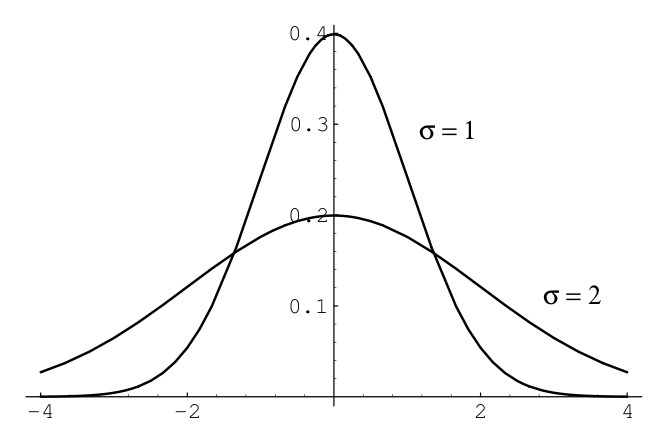
\includegraphics[width=0.6\columnwidth]{figs/intro/normal.png}
  \caption{\label{fig:normaldist} Normal density for two sets of parameter values.}
\end{center}
\end{figure}

Figure \ref{fig:normaldist} compares a plot of normal density for the cases $\mu=0$ and $\sigma=1$, and 
$\mu=0$ and  $\sigma=2$.


\subsection{Maximum Likelihood Estimation}
Until now we assumed that, for every distribution, the parameters $\theta$ are known and are used when we calculate $p(x|\theta)$. There are some cases where the values of the parameters are easy to infer, such as the probability $p$ of getting a head using a fair coin, used on a Bernoulli or Binomial distribution. However, in many problems, these values are complex to define and it is more viable to estimate the parameters using the data $x$. For instance, in the example above with the coin toss, if the coin is somehow tampered to have a biased behavior, rather than examining the dynamics or the structure of the coin to infer a parameter for $p$, a person could simply throw the coin $n$ times, count the number of heads $h$ and set $p=\frac{h}{n}$. By doing so, the person is using the data $x$ to estimate $\theta$.

With this in mind, we will now generalize this process by defining the probability $p(\theta|x)$ as the probability of the parameter $\theta$, given the data $x$. This probability is called {\bf likelihood} $\likelihood(\theta|x)$ and measures how well the parameter $\theta$ models the data $x$. The likelihood can be defined in terms of the distribution $f$ as
\begin{equation*}
\likelihood(\theta|x_1,...,x_n)=\prod_{i=1}^n f(x_i|\theta)
\end{equation*}
where $x_1,...,x_n$ are independently and identically distributed (i.i.d.) samples.

To understand this concept better, we go back to the tampered coin example again. Suppose that we throw the coin 5 times and get the sequence [1,1,1,1,1] (1=head, 0=tail). Using the Bernoulli distribution (see Section~\ref{bernoulli-eq}) $f$ to model this problem, we get the following likelihood values:
\begin{itemize}
\item $\likelihood(0,x) = f(1,0)^5 = 0^5 = 0$
\item $\likelihood(0.2,x) = f(1,0.2)^5 = 0.2^5 = 0.00032$
\item $\likelihood(0.4,x) = f(1,0.4)^5 = 0.4^5 = 0.01024$
\item $\likelihood(0.6,x) = f(1,0.6)^5 = 0.6^5 = 0.07776$
\item $\likelihood(0.8,x) = f(1,0.8)^5 = 0.8^5 = 0.32768$
\item $\likelihood(1,x) = f(1,1)^5 = 1^5 = 1$
\end{itemize}

If we get the sequence [1,0,1,1,0] instead, the likelihood values would be:
\begin{itemize}
\item $\likelihood(0,x) = f(1,0)^3f(0,0)^2 = 0^3\times 1^2 = 0$
\item $\likelihood(0.2,x) = f(1,0.2)^3f(0,0.2)^2 = 0.2^3\times 0.8^2 = 0.00512$
\item $\likelihood(0.4,x) = f(1,0.4)^3f(0,0.4)^2 = 0.4^3\times 0.6^2 = 0.02304$
\item $\likelihood(0.6,x) = f(1,0.6)^3f(0,0.6)^2 = 0.6^3\times 0.4^2 = 0.03456$
\item $\likelihood(0.8,x) = f(1,0.8)^3f(0,0.8)^2 = 0.8^3\times 0.2^2 = 0.02048$
\item $\likelihood(1,x) = f(1,1)^5 = 1^3\times 0^2 = 0$
\end{itemize}

We can see that the likelihood is the highest when the distribution $f$ with parameter $p$ is the best fit for the observed samples. Thus, the best estimate for $p$ according to $x$ would be the value for which $\likelihood(p,x)$ is the highest. 

The value of the parameter $\theta$ with the highest likelihood is called {\bf maximum likelihood estimate (MLE)} and is defined as
\begin{equation*}
\hat{\theta}_{mle}=argmax_{\theta}\likelihood(\theta|x)
\end{equation*}

Finding this for our example is relatively easy, since we can simply derivate the likelihood function to find the absolute maximum. For the sequence [1,0,1,1,0], the likelihood would be given as
\begin{equation*}
\likelihood(p,x) = f(1,p)^3f(0,p)^2 = p^3(1-p)^2
\end{equation*}

And the MLE estimate would be given by:
\begin{equation*}
\frac{\delta \likelihood(p,x)}{\delta p}=0
\end{equation*}
which resolves to
\begin{equation*}
p_{mle}=0.6
\end{equation*}

\begin{exercise}
Over the next couple of exercises we will make use of the Galton dataset, a dataset of heights of fathers and sons from the 1877 paper that first discussed the ``regression to the mean'' phenomenon. This dataset has 928 pairs of numbers.
\begin{itemize}
\item Use the \texttt{load()} function in the \texttt{galton.py} file to load the dataset. The file is located under the \texttt{lxmls/readers} folder. Type the following in your Python interpreter:
\begin{verbatim}
import galton as galton
GaltonData = galton.load()
\end{verbatim}
\item What are the mean height and standard deviation of all the people in the sample? What is the mean height of the fathers and of the sons?
\item Plot a histogram of all the heights (you might want to use the \texttt{plt.hist} function and the \texttt{ravel} method on arrays).
\item Plot the height of the father versus the height of the son.
\item You should notice that there are several points that are exactly the same (e.g., there are 21 pairs with the values 68.5 and 70.2). Use the \texttt{?} command in ipython to read the documentation for the \texttt{numpy.random.randn} function and add random jitter (i.e., move the point a little bit) to the points before displaying them. Does your impression of the data change?
\end{itemize}
\end{exercise}

\subsection{Conjugate Priors}
%\fbox
%{\begin{minipage}[h]{0.9\linewidth} 
\begin{definition}
let $\mathcal{F}= \{f_{X}(x|s), s \in \mathcal{X}\}$ be a class of likelihood functions; let $\mathcal{P}$ be a class of probability (density or mass) functions; if, for any $x$, any $p_{S}(s) \in \mathcal{P}$, and any $f_{X}(x|s) \in \mathcal{F}$, the resulting a posteriori probability function $p_{S}(s|x) = f_{X}(x|s)p_{S}(s)$ is still in $\mathcal{P}$, then $\mathcal{P}$ is called a conjugate family, or a family of {\bf conjugate priors}, for $\mathcal{F}$.
\end{definition}
%\end{minipage}}
%\gka{An example here for conjugate families}


\section{Numerical optimization}
Most problems in machine learning require minimization/maximization of functions (likelihoods, risk, energy, entropy, etc.,). Let $x^*$ be the value of $x$ which minimizes the value of some function $f(x)$. Mathematically, this is written as

\begin{equation*}
x^* = \argmin_x f(x)
\end{equation*}

In a few special cases, we can solve this minimization problem analytically in closed form (solving for optimal $x^{*}$ in  $\nabla_{x}f(x^{*})=0$), but in most cases it is too cumbersome (or impossible) to solve these equations analytically, and they must be tackled numerically. In this section we will cover some basic notions of numerical optimization. The goal is to provide the intuitions behind the methods that will be used in the rest of the school. There are plenty of good textbooks in the subject that you can consult for more information \citep{Nocedal1999,bertsekas1995np,boyd2004convex}.

The most common way to solve the problems when no closed form solution is available is to resort to an iterative algorithm. In this Section, we will see some of these iterative optimization techniques. These iterative algorithms construct a sequence of points $x^{(0)},x^{(1)},\ldots \in \text{domain}(f)$ such that hopefully $x^t = x^*$ after a number of iterations.
Such a sequence is called the {\bf minimizing sequence} for the problem.

\subsection{Convex Functions}

One important property of a function $f(x)$ is whether it is a \textbf{convex function} (in the shape of a bowl) or a \textbf{non-convex function}. Figures \ref{fig:convexfn} and \ref{fig:nonconvexfn} show an example of a convex and a non-convex function. Convex functions are particularly useful since you can guarantee that the minimizing sequence converges to the true global minimum of the function, while in non-convex functions you can only guarantee that it will reach a local minimum. 


 \begin{figure}[h]
 \begin{center}
     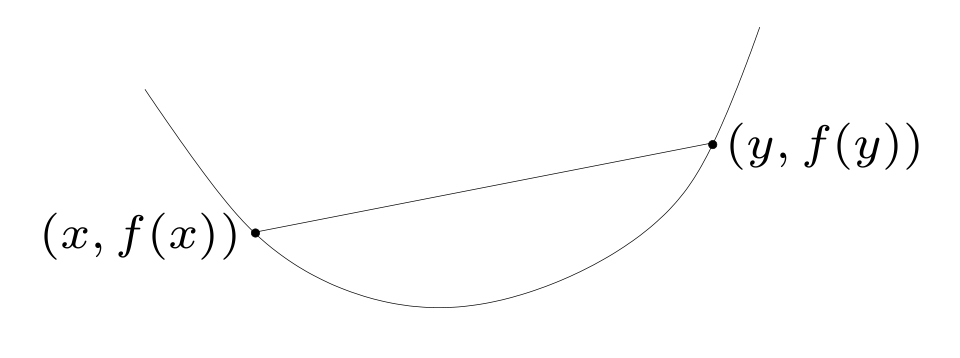
\includegraphics[width=0.6\columnwidth]{figs/intro/convexfn.png}
   \caption{\label{fig:convexfn} Illustration of a convex function. The line segment between any two points on the graph lies entirely above the curve.} 
     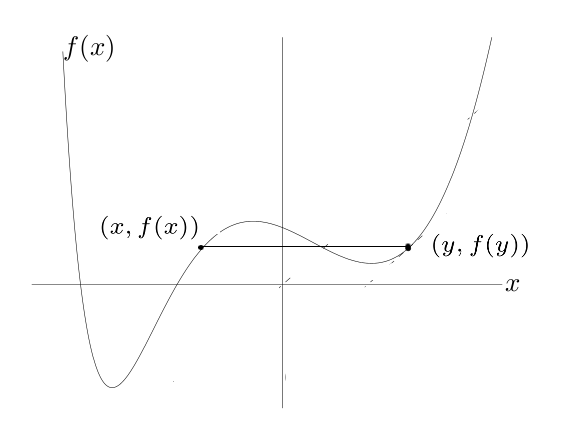
\includegraphics[width=0.5\columnwidth]{figs/intro/nonconvexfn.png}
   \caption{\label{fig:nonconvexfn} Illustration of a non-convex function. Note the line segment intersecting the curve. } 
 \end{center}
 \end{figure}


Intuitively, imagine dropping a ball on either side of Figure \ref{fig:convexfn}, the ball will roll to the bottom of the bowl independently from where it is dropped. This is the main benefit of a convex function. On the other hand, if you drop a ball from the left side of Figure \ref{fig:nonconvexfn} it will reach a different position than if you drop a ball from its right side. Moreover, dropping it from the left side will lead you to a much better (\emph{i.e.}, lower) place than if you drop the ball from the right side. This is the main problem with non-convex functions: there are no guarantees about the quality of the local minimum you find.

More formally, some concepts to understand about convex functions are:

\noindent A {\bf line segment} between points $x_{1}$ and $x_{2}$: contains all points such that 
\begin{equation*}
x=\theta x_{1} + (1-\theta)x_{2}
\end{equation*}
where $0\leq \theta \leq 1$.

\vspace{0.1in}
\noindent A {\bf convex set} contains the line segment between any two points in the set 
\begin{equation*}
x_{1}, x_{2} \in C,\hspace{0.12in} 0 \leq \theta \leq 1 \hspace{0.12in} \Rightarrow \hspace{0.12in} \theta x_{1} + (1-\theta)x_{2} \in C.
\end{equation*}

\vspace{0.1in}
\noindent A function $f: \mathbb{R}^{n}\rightarrow R$ is a {\bf convex function} if the domain of $f$ is a convex set and 
\begin{equation*}
f(\theta x + (1-\theta) y) \leq \theta f(x) + (1-\theta) f(y)
\end{equation*}

\noindent for all $x,y \in \text{domain of } f$, $0 \leq \theta \leq 1$

\subsection{Derivative and Gradient}

The \textbf{derivative} of a function is a measure of how the function varies with its input variables. Given an interval $[a,b]$ one can compute how the function varies within that interval by calculating the average slope of the function in that interval: 
\begin{equation}
\frac{f(b) - f(a)}{b-a}.
\end{equation}
The derivative can be seen as the limit as the interval goes to zero, and it gives us the slope of the function at that point.
\begin{equation}
\frac {\partial f}{\partial x} = \lim_{h = 0} \frac{f(x+h) - f(x)}{h} 
\end{equation}

\noindent Table \ref{tb::derivatives} shows derivatives of some functions that we will be using during the school.

\begin{table}[!h]
\begin{center}
\begin{tabular}{|l|l|}
\hline
Function $f(x)$& Derivative $\frac{\partial f}{\partial x}$\\
\hline
$x^2$ & $2x$\\
\hline
$x^n$ & $nx^{n-1}$\\
\hline
$\log(x)$ & $\frac{1}{x}$\\
\hline
$\exp(x)$ & $\exp(x)$\\
\hline
$\frac{1}{x}$ & $-\frac{1}{x^{2}}$\\
\hline
\end{tabular}
\end{center}
\caption{\label{tb::derivatives}Some derivative examples}
\end{table}

An important rule of derivation is the chain rule. Consider $h=f\circ g$, and $u=g(x)$, then:

\begin{equation}
\frac{\partial h}{\partial x}=\frac{\partial f}{\partial u}\cdot\frac{\partial g}{\partial x}
\end{equation}

\begin{example}

Consider the function $h(x)=\exp(x^{2})$, this can be decomposed as $h(x)=f(g(x))=f(u)=\exp(u)$, where $u=g(x)=x^{2}$ and has derivative $\frac{\partial h}{\partial x}=\frac{\partial f}{\partial u}\cdot \frac{\partial u}{\partial x}=\exp(u) \cdot 2x=\exp(x^{2}) \cdot 2x$

\end{example}

\begin{exercise}
Consider the function $f(x) = x^2$ and its derivative $\frac{\partial f} {\partial x}$. Look at the derivative of that function at points [-2,0,2], draw the tangent to the graph in that point $\frac{\partial f}{\partial x}\left(-2\right)=-4$, $\frac{\partial f}{\partial x}\left(0\right)=0$, and $\frac{\partial f}{\partial x}\left(2\right)=4$. For example, the tangent equation for $x=-2$ is $y=-4x - b$, where $b=f(-2)$. The following code plots the function and the derivatives on those points using matplotlib (See Figure \ref{fig:tangents}).

\begin{python}
a = np.arange(-5,5,0.01)
f_x = np.power(a,2)
plt.plot(a,f_x)

plt.xlim(-5,5)
plt.ylim(-5,15)

k= np.array([-2,0,2])
plt.plot(k,k**2,"bo")
for i in k:
    plt.plot(a, (2*i)*a - (i**2))

\end{python}

\begin{figure}[h]
\begin{center}
   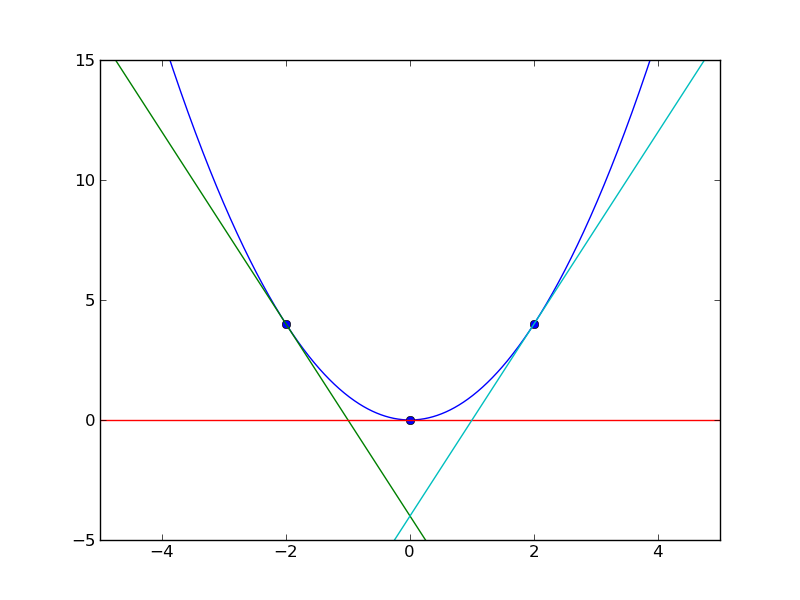
\includegraphics[width=0.6\columnwidth]{figs/intro/tangents.png}
 \caption{\label{fig:tangents} Illustration of the gradient of the
   function $f(x^2)$ at three different points $x = [-2,0.2]$. Note
   that at point $x = 0$ the gradient is zero which corresponds to the
 minimum of the function.}
\end{center}
\end{figure}

\end{exercise}

The \textbf{gradient} of a function is a generalization of the derivative concept we just saw before for several dimensions. Lets assume we have a function  $f(x)$ where $x \in \mathbb{R}^2$, so $x$ can be seen as a pair $x = [{x_1,x_2}]$. Then, the gradient measures the slope of the function in both directions: $\nabla_{x} f(x) = [\frac {\partial f}{\partial x_1},\frac {\partial f}{\partial x_2}]$.

\subsection{\label{gradient_methods} Gradient Based Methods}

Gradient based methods are probably the most common methods used for finding the minimizing sequence for a given function. The methods used in this class will make use of the function value $f(x)$ as well as the gradient of the function $\nabla_{x} f(x)$. The simplest method is the {\bf Gradient descent} method, an unconstrained first-order optimization algorithm.

The intuition of this method is as follows: You start at a given point $x_0$ and compute the gradient at that point $\nabla_{x_0} f(x)$. You then take a step of length $\eta$ on the direction of the negative gradient to find a new point: $x_1$ = $x_0 - \eta \nabla_{x_{0}}
f(x)$. Then, you compute the gradient at this new point, $\nabla_{x_1} f(x)$, and take a step of length $\eta$ on the direction of the negative gradient to find a new point: $x_2$ = $x_1 - \eta \nabla_{x_{1}} f(x)$. You proceed until you have reached a minimum (local or global). Recall from the previous subsection that you can identify the minimum by testing if the norm of the gradient is zero: $||\nabla f(x)|| = 0$.

There are several practical concerns even with this basic algorithm to ensure both that the algorithm converges (reaches the minimum) and that it does so in a fast way (by fast we mean the number of function and gradient evaluations).

\begin{itemize}
\item \textbf{Step Size $\eta$} A first question is how to find the step length $\eta$. One condition is that $eta$ should guarantee sufficient decrease in the function value. We will not cover these methods here but the most common ones are \textbf{Backtracking line search} or the \textbf{Wolf Line Search} \citep{Nocedal1999}.
\item \textbf{Descent Direction}  A second problem is that using the negative gradient as direction can lead to a very slow convergence. Different methods that change the descent direction by multiplying the gradient by a matrix $\beta$ have been proposed that guarantee a faster convergence. Two notable methods are the Conjugate Gradient (CG) and the Limited Memory Quasi Newton methods (LBFGS) \citep{Nocedal1999}.
\item \textbf{Stopping Criteria} Finally, it will normally not be possible to reach full convergence either because it will be too slow, or because of numerical issues (computers cannot perform exact arithmetic). So normally we need to define a stopping criteria for the algorithm. Three common criteria (that are normally used together) are: a maximum number of iterations; the gradient norm be smaller than a given threshold   $||\nabla f(x)|| \leq \eta_1$, or the normalized difference in the function value be smaller than a given threshold $\frac{|f(x_t) - f(x_{t-1})|}{\max(|f(x_t)|,|f(x_{t-1})|)} \leq \eta_2$
\end{itemize}

Algorithm \ref{alg:graddescent} shows the general gradient based algorithm. Note that for the simple gradient descent algorithm $\beta$ is the identity matrix and the descent direction is just the negative gradient of the function, $\beta = -\nabla f(x)$. Figure \ref{fig:graddescent} shows an illustration of the gradient descent algorithm.

\begin{algorithm}[h]
\caption{Gradient Descent\label{alg:graddescent}}
\begin{algorithmic}[1]
\STATE {\bf given} a starting point $x_{0}, i=0$
\STATE {\bf repeat}
\STATE \quad Compute step size $\eta$
\STATE \quad Compute descent direction $- \beta\nabla f(x_{i})$.
\STATE \quad $x_{i+1} \leftarrow x_{i} - \eta\beta\nabla f(x_{i})$
\STATE \quad $i \leftarrow i + 1$
\STATE {\bf until} stopping criterion is satisfied.
\end{algorithmic}
\end{algorithm}

\begin{figure}[h]
\begin{center}
   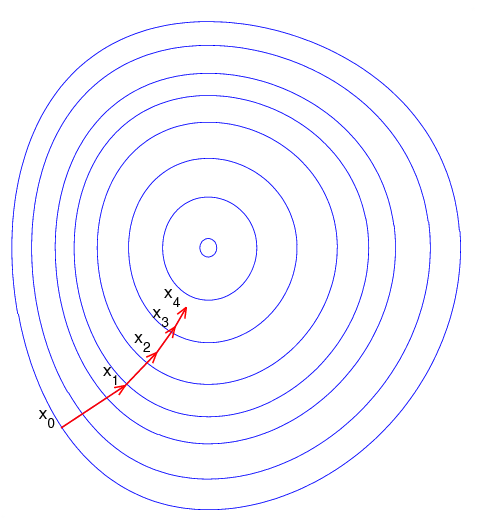
\includegraphics[width=0.6\columnwidth]{figs/intro/graddescent.png}
 \caption{\label{fig:graddescent} Illustration of gradient descent. The blue circles correspond to contours of the function (each blue circle is a set of points which have the same function value), while the red lines correspond to steps taken in the negative gradient direction.}
\end{center}
\end{figure}

% Gradient descent can work in any number of dimensions.  The process can also include {\bf line search} 
% to determine the locally optimal $\eta$ in each iteration. For non-differentiable functions, gradient 
% methods are ill-defined. Also, the procedure can take many iterations to converge to a local minimum 
% and methods based on Newton's method can be better alternatives. The main idea behind
% the iterative minimization techniques is find the locally best direction to move towards the (unknown) minimum. 
% While gradient descent moves in the direction of the negative gradient, other techniques like steepest 
% descent, conjugate descent, (L-)BGFS etc use other directions for update.

\begin{exercise}
Consider the function $f(x) = (x+2)^2 - 16 \exp\left( -(x-2)^2 \right)$.
Make a function that computes the function value given $x$.

\begin{python}
def get_y(x):
    return (x+2)**2 - 16*np.exp(-((x-2)**2))
\end{python}

Draw a plot around $x \in [-8,8]$.

\begin{python}
x = np.arange(-8,8,0.001)
y = map(lambda u: get_y(u),x)
plt.plot(x,y)
plt.show()
\end{python}

Calculate the derivative of the function $f(x)$, implement the function \emph{get\_grad(x)}.

\begin{python}
def get_grad(x):
    return (2*x+4)-16*(-2*x + 4)*np.exp(-((x-2)**2))
\end{python}

Use the method \emph{gradient\_descent} to find the minimum of this function. Convince yourself that the code is doing the proper thing. Look at the constants we defined. Note, that we are using a simple approach to pick the step size (always have the value step\_size) which is not necessarily correct.

\begin{python}
def gradient_descent(start_x,func,grad):
    # Precision of the solution
    prec = 0.0001
    #Use a fixed small step size
    step_size = 0.1
    #max iterations
    max_iter = 100
    x_new = start_x
    res = []
    for i in xrange(max_iter):
        x_old = x_new
        #Use beta egual to -1 for gradient descent 
        x_new = x_old - step_size * grad(x_new)
        f_x_new = func(x_new)
        f_x_old = func(x_old)
        res.append([x_new,f_x_new])
        if(abs(f_x_new - f_x_old) < prec):
            print "change in function values too small, leaving"
            return np.array(res)
    print "exceeded maximum number of iterations, leaving"
    return np.array(res)
\end{python}

Run the gradient descent algorithm starting from $x_0 = -8$ and plot the minimizing sequence.

\begin{python}
x_0 = -8
res = gradient_descent(x_0,get_y,get_grad)
plt.plot(res[:,0],res[:,1],'+')
plt.show()
\end{python}


\begin{figure}[h]
\begin{center}
   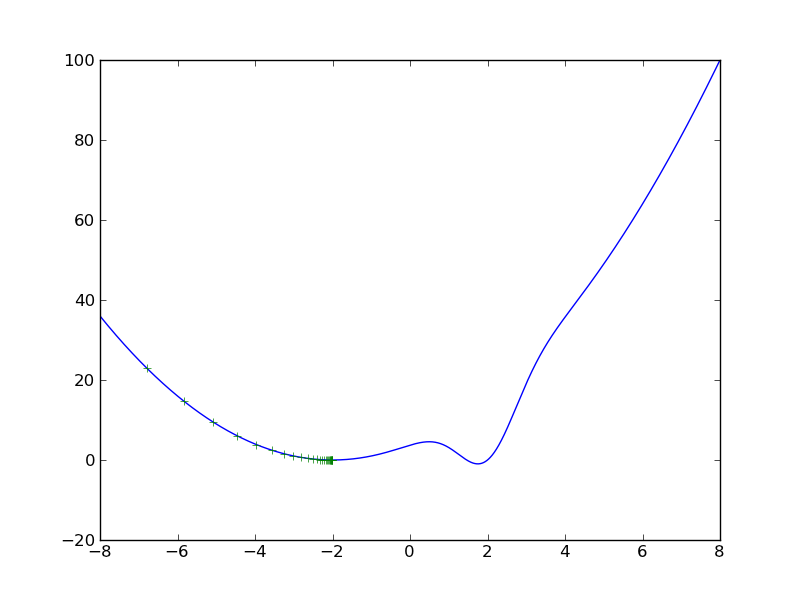
\includegraphics[width=1\columnwidth]{figs/intro/gradex1.png}
 \caption{\label{fig:gradex1} Example of running gradient descent
   starting on point $x_0 = -8$ for function $f(x) = (x+2)^2 - 16
   \exp\left( -(x-2)^2 \right)$. The function is represented in blue,
   while the points of the minimizing sequence are displayed as green
   plus signs.}
\end{center}
\end{figure}


Figure \ref{fig:gradex1} shows the resulting minimizing sequence. Note that the algorithm converged to a minimum, but since the function is not convex it converged only to a local minimum.

Now try the same exercise starting from the initial point $x_0 = 8$.

\begin{python}
x_0 = 8
res = gradient_descent(x_0,get_y,get_grad)
plot(res[:,0],res[:,1],'+')
\end{python}


\begin{figure}[h]
\begin{center}
   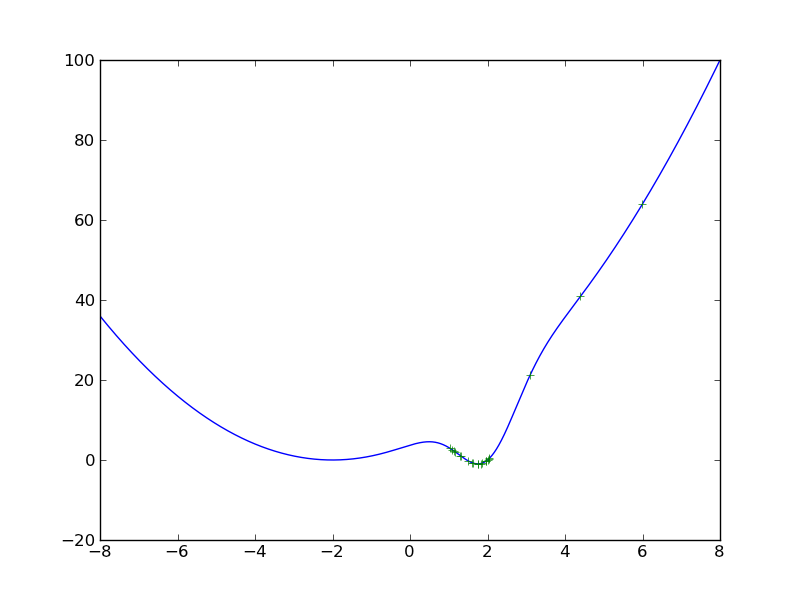
\includegraphics[width=1\columnwidth]{figs/intro/gradex2.png}
 \caption{\label{fig:gradex2} Example of running gradient descent
   starting on point $x_0 = 8$ for function $f(x) = (x+2)^2 - 16
   \exp\left( -(x-2)^2 \right)$. The function is represented in blue,
   while the points of the minimizing sequence are displayed as green
   plus signs.}
\end{center}
\end{figure}


Figure \ref{fig:gradex2} shows the resulting minimizing sequence. Note that now the algorithm converged to the global minimum. However, note that to get to the global minimum the sequence of points jumped from one side of the minimum to the other. This is a consequence of using a wrong step size (in this case too large). Repeat the previous exercise changing both the values of the step-size and the precision. What do you observe?
\end{exercise}

During this school we will rely on the numerical optimization methods provided by Scipy (scientific computing library in python), which are very efficient implementations.


% \begin{exercise}
% Consider the linear regression problem (ordinary least squares), with a
% single response variable

% \[
% y = x^T w + \varepsilon
% \]

% The \emph{linear regression problem} is, given a set $\{ y^{(i)} \}_i$ of
% samples of $y$ and the corresponding $\vect{x}^{(i)}$ vectors, estimate
% $\vect{w}$ to minimise the sum of the $\varepsilon$ variables. Traditionally
% this is solved analytically to obtain a closed form solution (although this is
% \textbf{not the way in which it should be computed}, linear algebra packages
% have an optimised solver, with numpy, use \code{numpy.linalg.lstsq}).

% Alternatively, we can define the error function for each possible $\vect{w}$:

% \[
% e(\vect{w}) = \sum_i \left( {\vect{x}^{(i)}}^T \vect{w} - y^{(i)} \right)^2.
% \]

% \begin{enumerate}
% \item Derive the gradient of the error $\pd{e}{w_j}$.
% \item Implement a solver based on this for two dimensional problems (i.e.,
% $\vect{w} \in R^2$).
% \item Use this method on the Galton dataset from the previous exercise to
% estimate the relationship between father and son's height. Try two formulas
% \begin{equation}
% s = f w_1 + \varepsilon,
% \label{}
% \end{equation}
% where $s$ is the son's height, and $f$ is the father heights; and
% \begin{equation}
% s = f w_1 + 1w_0 + \varepsilon
% \label{}
% \end{equation}
% where the input variable is now two dimensional: $(f,1)$. This allows the
% intercept to be non-zero.
% \item Plot the regression line you obtain with the points from the previous
% exercise.
% \item Use the \texttt{np.linalg.lstsq} function and compare to your solution.
% \end{enumerate}
% \end{exercise}



%Basic concepts of numerical optimization.

%\begin{itemize}
%\item - Gradient base methods, gradient descent, its problems,
%  conjugate and lbfgs. Can use routines from python, make example with
%  Gaussian with different variates and show the behavior.
%\item convex functions vs non convex functions, very brief, convex
%  function is like a bowl, if you drop a ball from the top it will
%  reach the bottom, Non-convex several bottom, will reach one of them.
%\item Gradient, sub-gradient generalization
%\end{itemize}


% \subsection{Matrix Derivatives}

% In subsection we finalize by showing some basic formulas for the
% gradient of matrix:

% \begin{itemize}
% \item For vectors $a$ and $x$, $\frac{\partial a^{T} x}{\partial x}= a$
% \item For vectors $a$ and $x$ and matrix $A$, $\frac{\partial a^{T}Ab}{\partial A} = ab^{T}$
% \item For vectors $a$ and $x$ and matrix $A$, $\frac{\partial a^{T}A^{T}b}{\partial A} =  ba^{T}$
% \end{itemize}

% {\bf The Gradient: }Suppose that $f:\mathbb{R}^{m\times n} \rightarrow\mathbb{R}$ is a function that takes as input, a matrix $A$
% of size $m\times n$ and returns a real value. Then the {\bf gradient} of $f$ (with respect to $A\in \mathbb{R}^{m\times n}$)
% is the matrix of partial derivatives, defined as:
% \begin{equation*}
% \nabla_{A}f(A)\in \mathbb{R}^{m\times n} = \left[\begin{array}{cccc}
% \frac{\partial f(A)}{\partial A_{11}} & \frac{\partial f(A)}{\partial A_{12}} & \ldots & \frac{\partial f(A)}{\partial A_{1n}} \\
% \frac{\partial f(A)}{\partial A_{21}} & \frac{\partial f(A)}{\partial A_{22}} & \ldots & \frac{\partial f(A)}{\partial A_{2n}} \\
% \vdots & \vdots &\ddots & \vdots \\
% \frac{\partial f(A)}{\partial A_{m1}} & \frac{\partial f(A)}{\partial A_{m2}} & \ldots & \frac{\partial f(A)}{\partial A_{mn}} \\
% \end{array}\right].
% \end{equation*}

% The gradient is defined {\em only} if the function is real-valued, that is, if it returns a scalar value. Some 
% important properties:

% \begin{itemize}
% \item $\nabla_{x}(f(x) + g(x)) = \nabla_{x}f(x) + \nabla_{x}g(x)$.
% \item For $t \in \mathbb{R}$, $\nabla_{x}(tf(x))= t\nabla_{x}f(x)$.
% \item Let $f:\mathbb{R}^{m} \rightarrow \mathbb{R}$ be the function defined by $f(z)=z^{T}z$, $\nabla_{z}f(z)=2z$.
% \end{itemize}
% {\bf The Hessian:} Suppose that $f:\mathbb{R}^{n}\rightarrow\mathbb{R}$ is a function that takes a vector in $\mathbb{R}^{n}$ and
% returns a real number, then the {\em Hessian} matrix with respect to $x$, written $\nabla_{x}^{2}f(x)$ (or $H$) is the $n\times n$
% matrix of partial derivatives,

% \begin{equation*}
% \nabla_{x}^{2}f(x) \in \mathbb{R}^{n\times n}= \left[\begin{array}{cccc}
% \frac{\partial^{2}f(x)}{\partial x_{1}^{2}} & \frac{\partial^{2}f(x)}{\partial x_{1} \partial x_{2}} & \ldots &  \frac{\partial^{2}f(x)}{\partial x_{1} \partial x_{n}} \\
% \frac{\partial^{2}f(x)}{\partial x_{2} \partial x_{1}} & \frac{\partial^{2}f(x)}{\partial x_{2}^{2}} & \ldots &  \frac{\partial^{2}f(x)}{\partial x_{2} \partial x_{n}} \\
% \vdots & \vdots & \ddots & \vdots \\
% \frac{\partial^{2}f(x)}{\partial x_{n} \partial x_{1}} & \frac{\partial^{2}f(x)}{\partial x_{n}\partial x_{2}} & \ldots &  \frac{\partial^{2}f(x)}{\partial x_{n}^{2}} 

% \end{array}\right].
% \end{equation*}

% Note that the Hessian is always symmetric, since
% \begin{equation*}
% \frac{\partial^{2}f(x)}{\partial x_{i}\partial x_{j}} =\frac{\partial^{2}f(x)}{\partial x_{j}\partial x_{i}}.
% \end{equation*}



%%% Local Variables: 
%%% mode: latex
%%% TeX-master: "../../guide"
%%% End: 







%%% Local Variables: 
%%% mode: latex
%%% TeX-master: "../../guide"
%%% End: 
